\chapter{Gantt Chart}
\setlength{\parindent}{15pt}
\label{ch:gant_char}

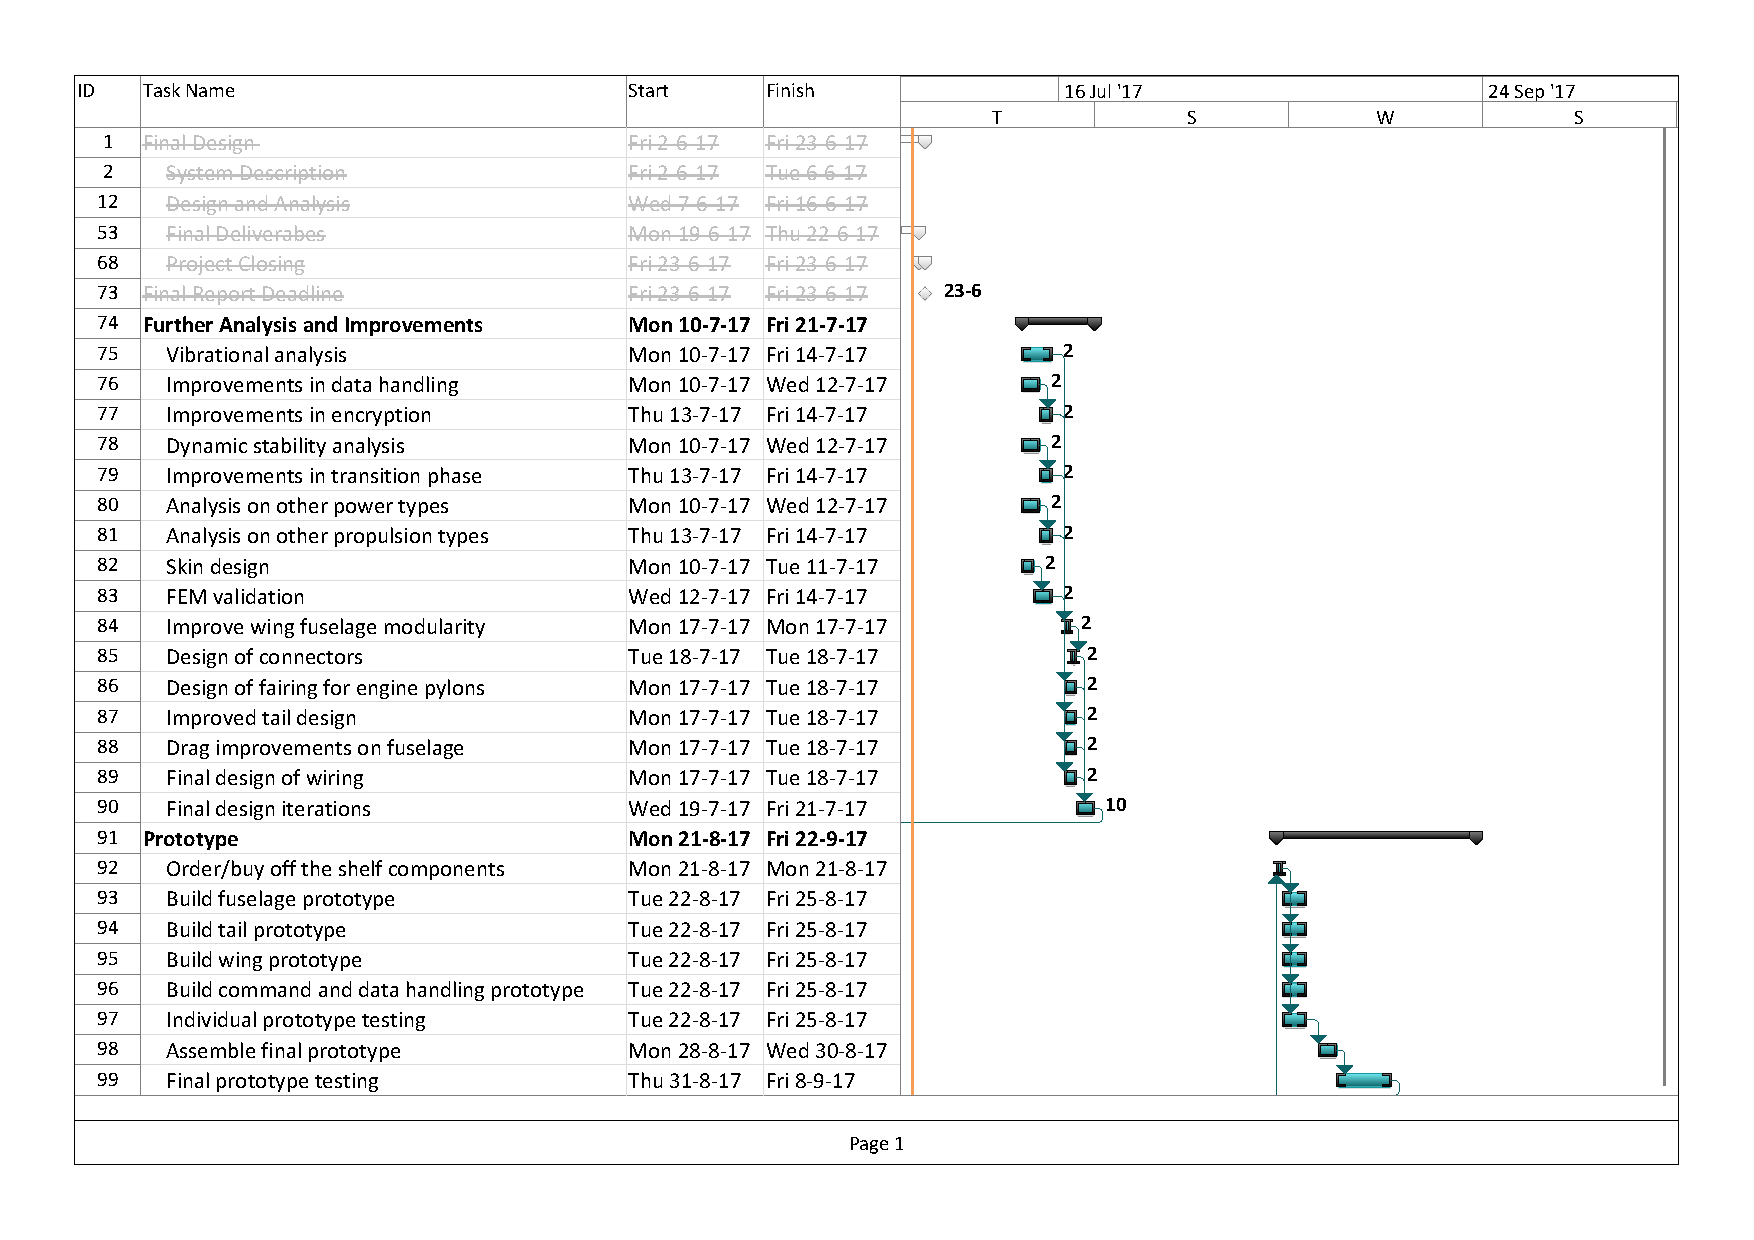
\includepdf[pages=1,fitpaper, scale=0.85,pagecommand={}]{Appendices/Figures/ProjectGantt1.pdf}
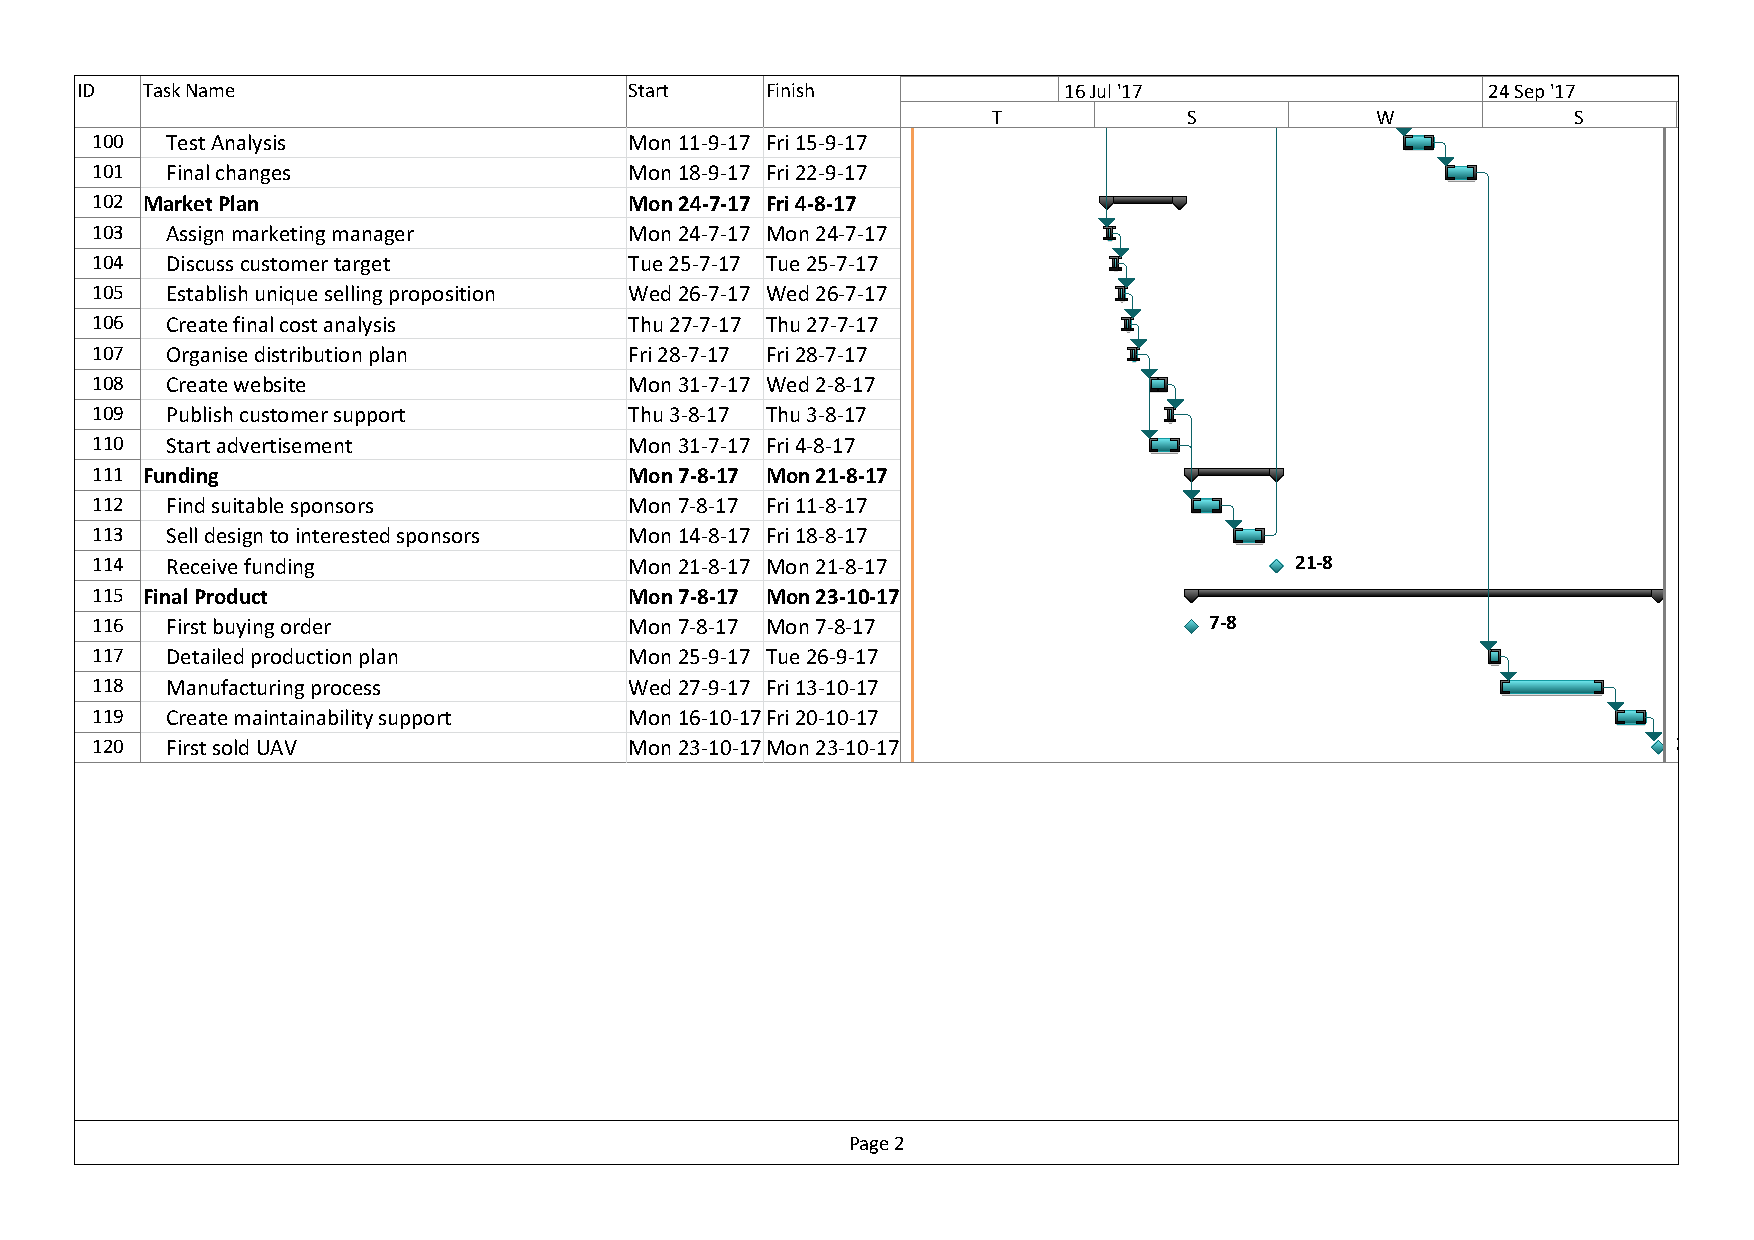
\includepdf[pages=1,fitpaper, scale=0.85,pagecommand={}]{Appendices/Figures/ProjectGantt2.pdf}

\chapter{Design Parameters}

\begin{table}[htb]
\centering
\caption{Center of Gravity Breakdown}
\label{tab:cgbreakdown}
\begin{tabular}{lrrr}
\toprule
\textbf{Subsystem} & \textbf{Mass [kg]} & \textbf{Minimum c.g. Location [m]} & \textbf{Maximum c.g. Location [m]} \\ \midrule
Wing & 2.5 & 0.60 & 0.60 \\ \hdashline
Tail & 1.35 & 1.68 & 1.68 \\ \hdashline
Battery 1 & 2.8 & 0.19 & 0.19 \\ \hdashline
Battery 2 & 5.4 & 0.35 & 0.35 \\ \hdashline
Payload & 6.2 & 0.4 & 0.8 \\ \hdashline
Fuselage & 2.30 & 0.9 & 0.9 \\ \hdashline
Avionics & 0.4 & 0.3 & 0.3 \\ \hdashline
Propulsion & 2.39 & 0.79 & 0.79 \\ \midrule
Total & 23.38 & 0.55 & 0.74 \\ \bottomrule
\end{tabular}
\end{table}

%table with aerodynamic values used in equations (Clalpha,..)

\chapter{Design Overview}
\label{ch:add_catia}

\begin{figure}[H]
    \centering
    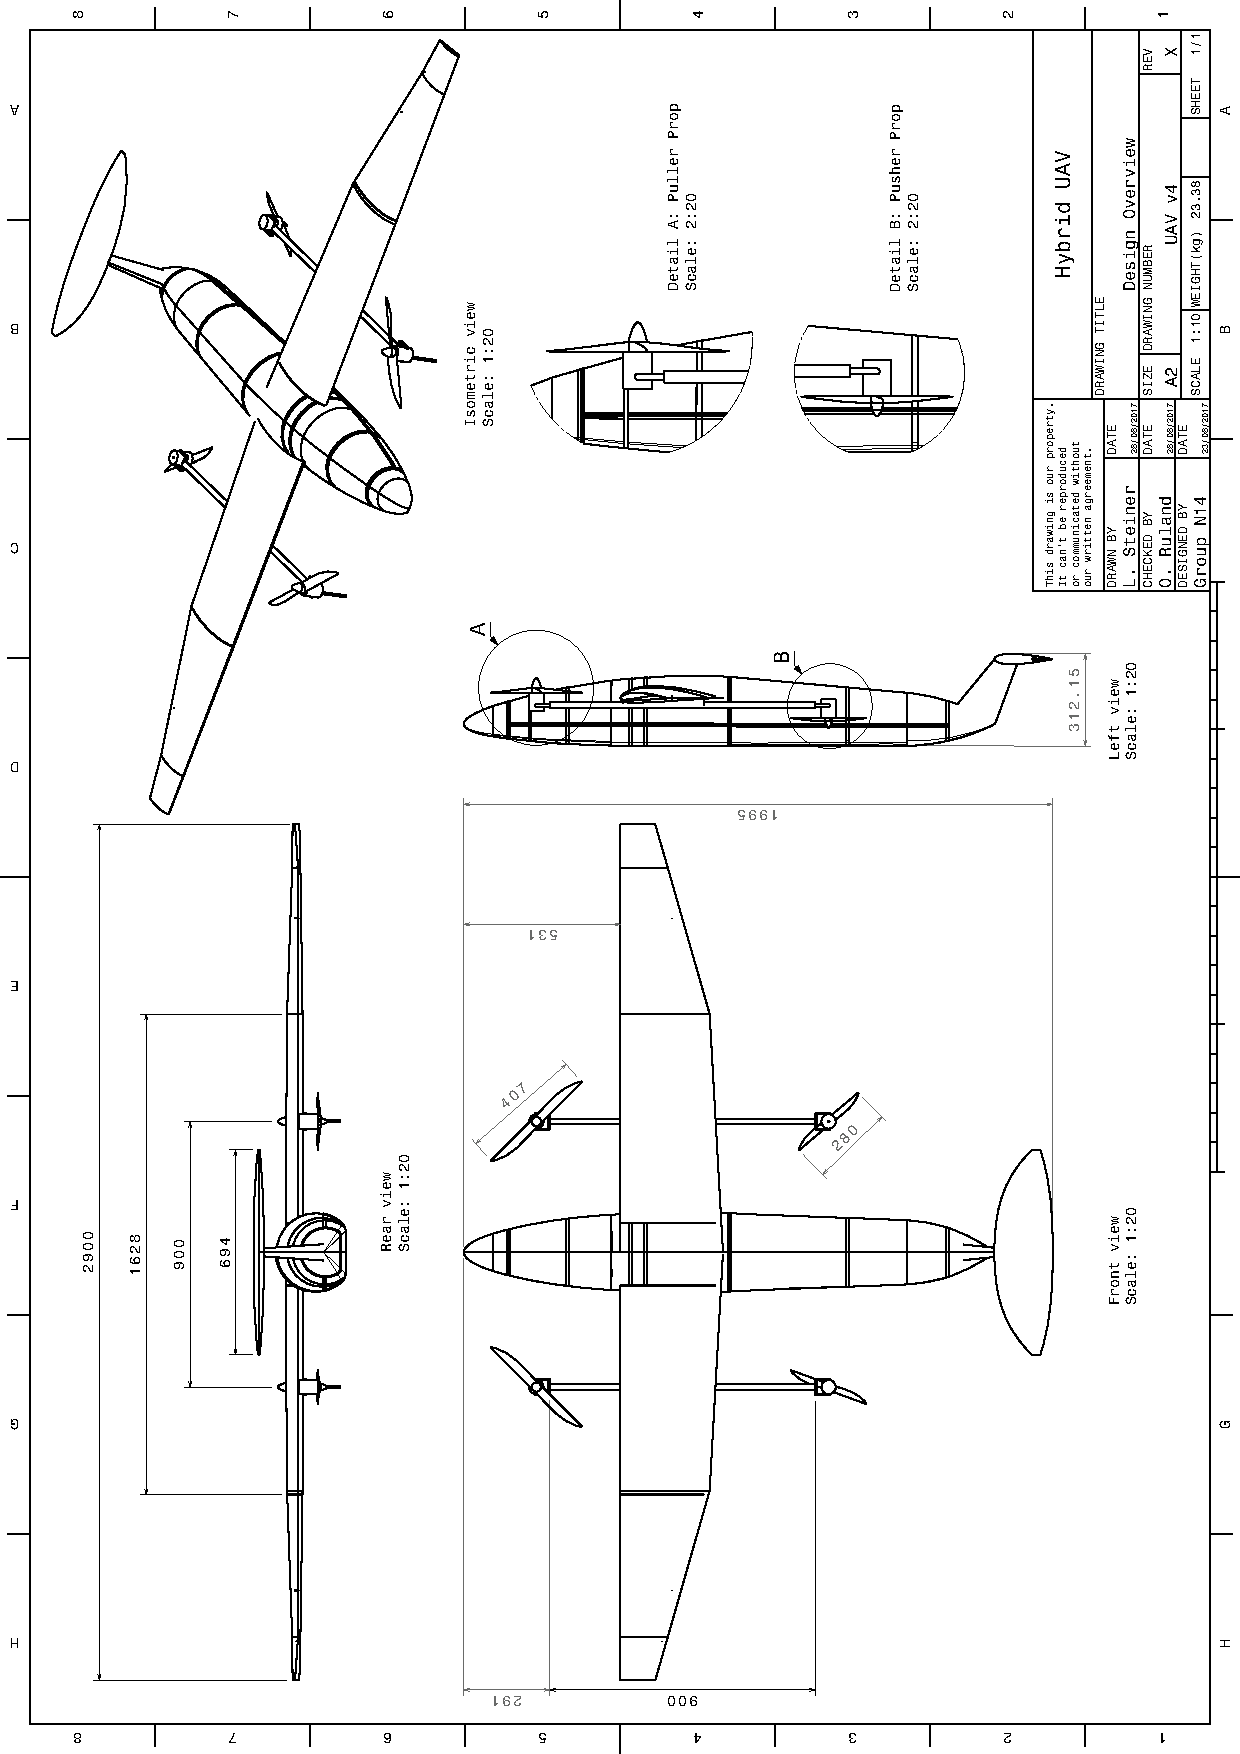
\includegraphics[width=\textwidth]{Appendices/Figures/overview_A4}
    \caption{Task Division Tool, General Tab}
    \label{fig:overview_A4}
\end{figure}




\chapter{Task Division Tool}
\setlength{\parindent}{15pt}
\label{ch:task_divi}

\begin{figure}[H]
    \centering
    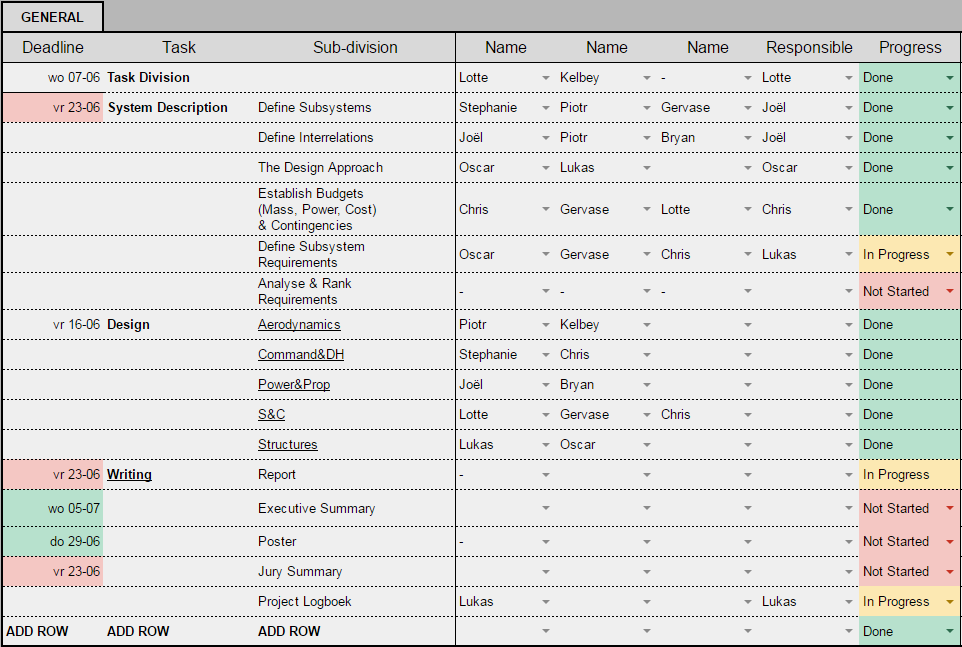
\includegraphics[scale=0.6]{Appendices/Figures/Taskdivisiongeneral}
    \caption{Task Division Tool, General Tab}
    \label{fig:task_divi_tool_gene}
\end{figure}

\begin{figure}[H]
    \centering
    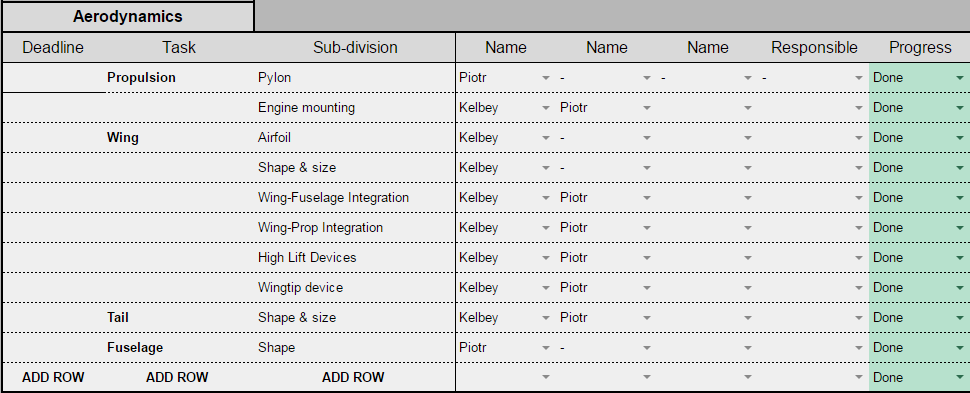
\includegraphics[scale=0.6]{Appendices/Figures/Taskdivisiondepartment}
    \caption{Task Division Tool, Department Tab}
    \label{fig:task_divi_tool_depa}
\end{figure}

\begin{figure}[H]
    \centering
    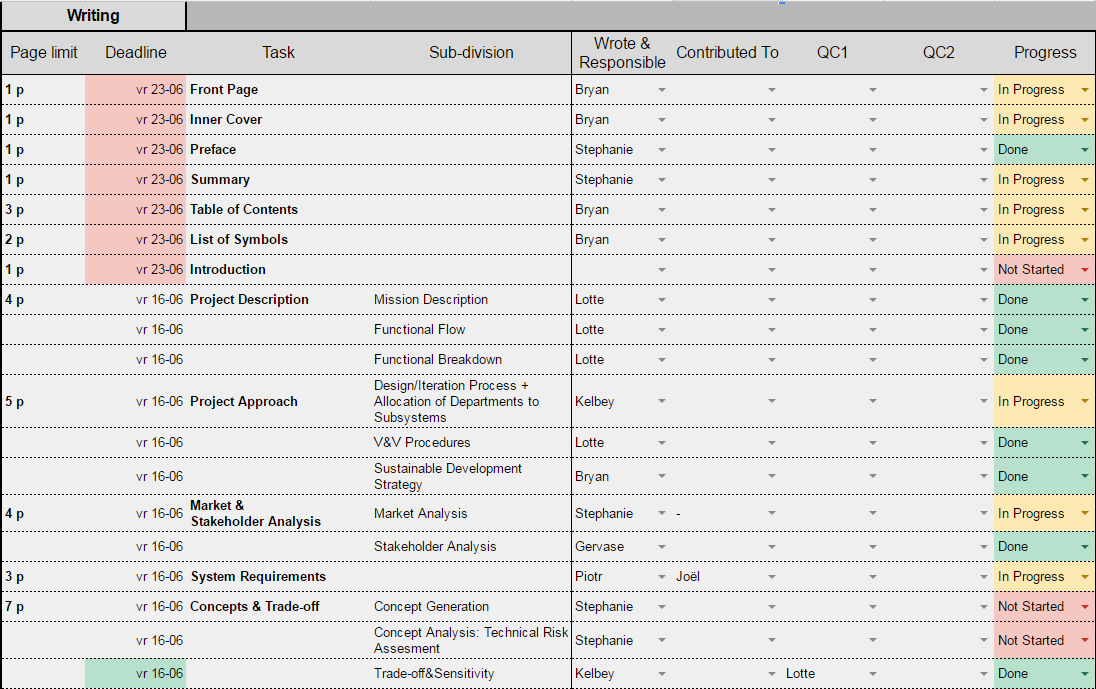
\includegraphics[scale=0.6]{Appendices/Figures/Taskdivisionwriting}
    \caption{Task Division Tool, Part of Writing Tab}
    \label{fig:task_divi_tool_writ}
\end{figure}

\chapter{Master Set Tool}
\setlength{\parindent}{15pt}
\label{ch:mast_set}

\begin{figure}[H]
    \centering
    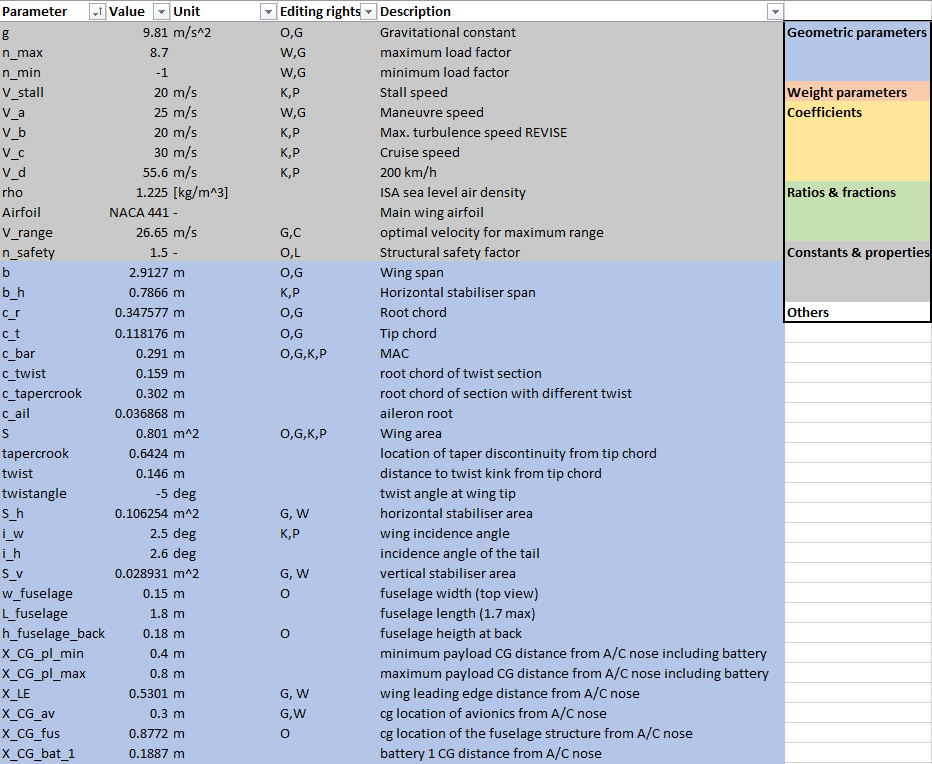
\includegraphics[scale=0.6]{Appendices/Figures/masterset}
    \caption{Portion of the Master Set}
    \label{fig:port_mast_set}
\end{figure}